Nesta seção será descrito o diagrama de máquina de estados, presente no SysML e também no UML. Ele é um digrama que apresenta as mudanças de estado de uma certa entidade, indicando os eventos responsáveis pelas transições entre estados.

%\subsubsection{O que é o diagrama de máquinas de estados}
%texto

\subsubsection{Estrutura dos diagramas de máquinas de estado}
\begin{figure}[H]
\centering
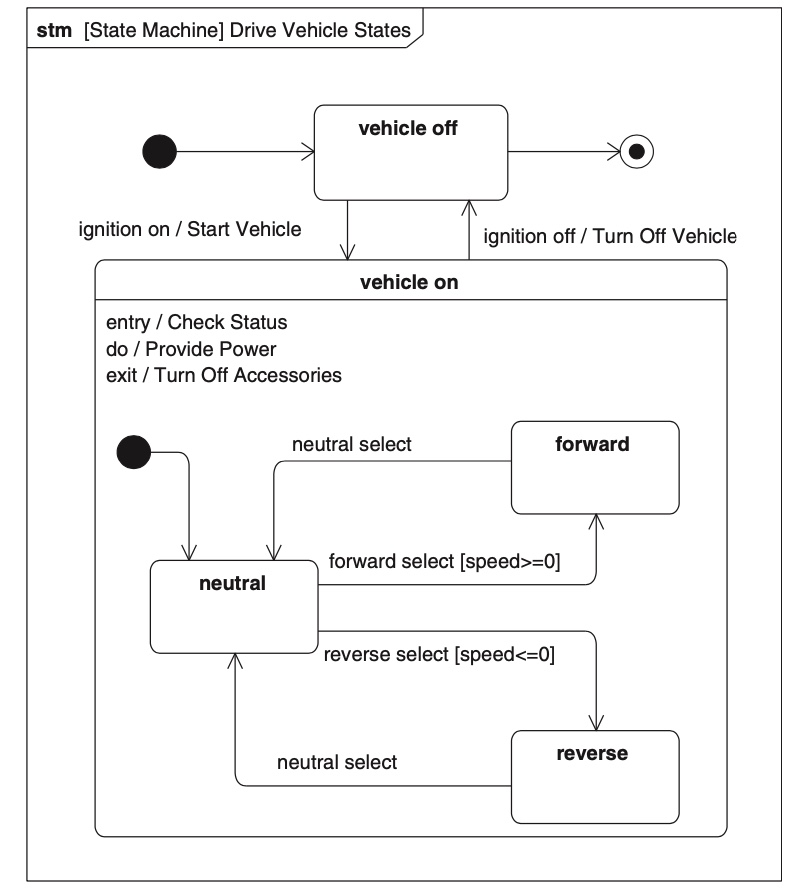
\includegraphics[width=0.75\textwidth]{figures/diagrama-maquina-estados.jpeg}
\caption{Diagrama Máquina de Estados}
\end{figure}
texto

\subsubsection{Onde são utilizados com frequência}
texto